\begin{pastexam}[label={px:ntu-107-bime-ds-05}]{臺大生機所 107 學年度 第 5 題}
（程式設計、分析）

(20\%) (a) Please implement a pseudocode function that performs the nearest neighbor search in a
\textbf{\textit{k}-d tree} with $k$=2 (find the closest point among $N$ 2-dimensional points to the
query point). (b) Analyze the complexity of your code.
\end{pastexam}

\begin{pastsoln}
$k$-d 樹資結書沒有專節，它是二元搜尋樹推廣到 $k$ 維：每個節點存一個點，並且用某一個座標把空間
切成兩半。 $k = 2$ 時一層用 $x$ 座標切、下一層用 $y$ 座標切，交替下去。 以下先說清楚樹的定義，
再寫最近點搜尋。

\textbf{樹的定義}。 每個節點 $t$ 有：點 $t.\mathit{pt}$（座標 $t.\mathit{pt}[0]$、$t.\mathit{pt}[1]$），
切的維度 $t.\mathit{axis}$（深度為偶數的節點是 $0$，奇數是 $1$），以及 $t.\mathit{left}$、
$t.\mathit{right}$。 令 $a = t.\mathit{axis}$，規定：左子樹的點都滿足 $\mathit{pt}[a] < t.\mathit{pt}[a]$，
右子樹的點都滿足 $\mathit{pt}[a] \ge t.\mathit{pt}[a]$。 也就是說，節點 $t$ 用直線
「第 $a$ 個座標 $= t.\mathit{pt}[a]$」把它負責的區域切成兩塊。 建樹時每次取第 $a$ 個座標的中位數當
節點，左右各分一半，樹高約 $\lg N$。

\textbf{(a) 最近點搜尋}。 距離用平方比較就好（不必開根號）。 想法和在二元搜尋樹找一個鍵值一樣：先往
查詢點 $q$ 所在的那一邊走（近的那一邊），走回來時再判斷另一邊（遠的那一邊）\textbf{有沒有可能}有更近
的點。 遠的那一邊的點都在切線的另一側，它們到 $q$ 的距離至少是 $q$ 到切線的距離
$|q[a] - t.\mathit{pt}[a]|$；這個距離已經不小於目前找到的最近距離，就整棵跳過。

\begin{pseudo}{2-d 樹的最近點搜尋}
\Function{Nearest}{$T, q$}
    \State $\mathit{best} \gets \NIL$; $\mathit{bestd} \gets \infty$ \Comment{目前最近的點和它的距離平方}
    \State \Call{NN}{$T.\mathit{root}, q$}
    \State \Return $\mathit{best}$
\EndFunction
\Statex
\Procedure{NN}{$t, q$}
    \If{$t = \NIL$}
        \State \Return
    \EndIf
    \State $d \gets (t.\mathit{pt}[0] - q[0])^2 + (t.\mathit{pt}[1] - q[1])^2$
    \If{$d < \mathit{bestd}$}
        \State $\mathit{best} \gets t.\mathit{pt}$; $\mathit{bestd} \gets d$
    \EndIf
    \State $a \gets t.\mathit{axis}$; $\delta \gets q[a] - t.\mathit{pt}[a]$ \Comment{$q$ 在切線的哪一側、多遠}
    \If{$\delta < 0$}
        \State $\mathit{near} \gets t.\mathit{left}$; $\mathit{far} \gets t.\mathit{right}$
    \Else
        \State $\mathit{near} \gets t.\mathit{right}$; $\mathit{far} \gets t.\mathit{left}$
    \EndIf
    \State \Call{NN}{$\mathit{near}, q$} \Comment{先找 $q$ 所在的那一邊}
    \If{$\delta^2 < \mathit{bestd}$} \Comment{以 $q$ 為圓心的圓跨過切線}
        \State \Call{NN}{$\mathit{far}, q$}
    \EndIf
\EndProcedure
\end{pseudo}

$\mathit{best}$、$\mathit{bestd}$ 是 \proc{Nearest} 和 \proc{NN} 共用的變數（用 C 寫時可以傳指標）。

\textbf{正確性}。 只要說明第 17 行跳過的子樹裡不可能有比 $\mathit{best}$ 更近的點；其他的點都會被
第 8 行看到。 設 $a = t.\mathit{axis}$，$r$ 是 $\mathit{far}$ 子樹裡的任一點。
\begin{itemize}
\item $\delta < 0$（$q[a] < t.\mathit{pt}[a]$）：$\mathit{far}$ 是右子樹，$r[a] \ge t.\mathit{pt}[a]$，所以
$r[a] - q[a] \ge t.\mathit{pt}[a] - q[a] = |\delta|$。
\item $\delta \ge 0$（$q[a] \ge t.\mathit{pt}[a]$）：$\mathit{far}$ 是左子樹，$r[a] < t.\mathit{pt}[a]$，所以
$q[a] - r[a] > q[a] - t.\mathit{pt}[a] = \delta$。
\end{itemize}
兩種情形都有 $\mathrm{dist}(r, q)^2 \ge (r[a] - q[a])^2 \ge \delta^2$。 第 17 行不成立時
$\delta^2 \ge \mathit{bestd}$，而 $\mathit{bestd}$ 之後只會變小或不變，所以 $r$ 不會比最後的答案更近，
跳過它不影響結果。 歸納下去，\proc{Nearest} 回傳的 $\mathit{best}$ 是距離最小的點（有好幾個一樣近時，
回傳其中最先找到的一個）。

例：六個點 $(2,3)$、$(5,4)$、$(9,6)$、$(4,7)$、$(8,1)$、$(7,2)$ 建成的 2-d 樹如下（根用 $x$ 座標切，
第二層用 $y$ 座標切）：
\begin{center}
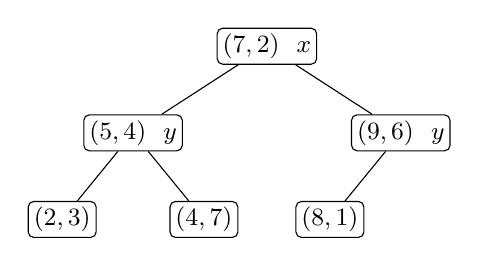
\begin{tikzpicture}[v/.style={draw,rounded corners=2pt,inner sep=2pt,font=\small},level distance=1.1cm,
  level 1/.style={sibling distance=3.4cm},level 2/.style={sibling distance=1.8cm}]
\node[v] {$(7,2)$ \ $x$}
  child {node[v] {$(5,4)$ \ $y$} child {node[v] {$(2,3)$}} child {node[v] {$(4,7)$}}}
  child {node[v] {$(9,6)$ \ $y$} child {node[v] {$(8,1)$}} child[missing]};
\end{tikzpicture}
\end{center}
查 $q = (9,2)$：
\begin{itemize}
\item 根 $(7,2)$：距離平方 $4$，$\mathit{best} = (7,2)$。 $\delta = 9 - 7 = 2 \ge 0$，先走右子樹。
\item $(9,6)$：距離平方 $16$，不更新。 $\delta = 2 - 6 = -4 < 0$，先走左子樹。
\item $(8,1)$：距離平方 $1 + 1 = 2 < 4$，$\mathit{best} = (8,1)$，$\mathit{bestd} = 2$。
\item 回到 $(9,6)$：$\delta^2 = 16 \ge 2$，不看右子樹（本來就是空的）。
\item 回到根：$\delta^2 = 4 \ge 2$，整個左子樹跳過。
\end{itemize}
答案 $(8,1)$，只看了 $3$ 個點。

\textbf{(b) 複雜度}。 每次呼叫 \proc{NN}（不含遞迴）是常數時間，所以時間和被拜訪的節點數成正比。
\begin{itemize}
\item \textbf{建樹}：每層用線性時間選中位數（資結書第~16~章）把點分兩半，
$T(N) = 2T(N/2) + \Theta(N) = \Theta(N \lg N)$；樹高 $\lfloor \lg N \rfloor + 1$，空間 $\Theta(N)$。
\item \textbf{搜尋的最好情形}：每個節點的遠側都被剪掉，只走一條根到葉的路徑，$\Theta(\lg N)$。
\item \textbf{最壞情形}：$\Theta(N)$，所有節點都要看。 例如 $N$ 個點平均分布在以 $q$ 為圓心、半徑 $\rho$
的圓周上：第一個看到的點就讓 $\mathit{bestd} = \rho^2$，但除了最左、最右、最上、最下那幾個點，每條切線
到 $q$ 的距離都小於 $\rho$，第 17 行幾乎每次都成立，遠側一直剪不掉。 這時和暴力比較每一個點一樣慢。
\item \textbf{一般情形}：點大致均勻分布時，以 $q$ 為圓心、半徑為答案距離的圓只會碰到常數個葉節點
的區域，期望拜訪 $O(\lg N)$ 個節點（Friedman、Bentley、Finkel，1977）。 例如 $N = 10^5$ 個均勻隨機的點，
一次查詢平均只看二十幾個節點。
\end{itemize}
額外空間是遞迴深度，等於樹高 $O(\lg N)$（樹建得平衡時）。 和不建樹、直接比較 $N$ 個點的 $\Theta(N)$
相比，建一次樹花 $\Theta(N \lg N)$，之後每次查詢通常只要 $O(\lg N)$，查詢次數多時划算。
\end{pastsoln}
